\section{Introduction}
\label{sec:db:intro}


The following chapter describes a procedure for searching for searching for a dark boson, \db, of
an unknown mass and lifetime\footnote{
  Throughout this chapter, the symbol \db shall denote a general dark boson and all references to
  a \Kstarz will be implicitly referencing the $K^*(892)^0$; unless explicitly stated otherwise.
}.
A fully frequentest method is applied to the dimuon distribution of \btokstrmumu candidates,
to search for an excess of events above the \sm background, \db consistent with a \db decaying via
\dbtomumu.
Lifetime information is added by searching for an excess of dimuon candidates in two lifetime bins:
one prompt, and one displaced.


Chapter~\ref{ch:theory} explains that the \sm cannot explain \dm, which is evidenced by
numerous experimental observations, and that
little is known about dark matter except that it interacts with the \sm sector only, or at least
predominantly, gravitationally and is therefore not directly visible to astronomical observations.
A possible extension to the \sm is to introduce a dark sector, which can contain a rich variety of
distinct particles operating through forces that are hitherto unknown.
Dark sector particles would be gauge singlet states with respect to the \sm, and
only be able to communicate with known particles via weakly interacting messenger particles
through one of four \emph{portals}: the vector, axion, Higgs, and neutrino portals.
Interaction terms for messengers in each of these portals are given in
\Table{tab:db:overview}.
In most dark sector models, the only way that a \db can be observed is if it mixes with a \sm
particle, and the superpostition of the two states decays into, in this case, a dimuon pair.


\begin{table}
  \caption[Summary of dark boson portals]
  {
    %from 1311.0029
    A summary of portals through which a new dark boson could operate.
    Terms are defined as:
    %$F_{\mu\nu}$ is the Yang-Mills field;
    $F_{\mu\nu}$ is the field strength tensor of the photon;
    $F^\prime_{\mu\nu}$ is the dark photon field;
    $\epsilon$ characterizes mixing between the \sm and the dark photon;
    $a$ is axion field;
    $f_a$ is scale at which Peccei-Quinn global $U(1)$ symmetry is spontaneously broken;
    $G_{\mu\nu}$ is the gluon field strength tensor;
    $S$ is a dark scalar field with coupling strengths $\mu$ and $\lambda$ to the Higgs field;
    and $N$ is the sterile neutrino which couples to a $H$ with a strength $Y_N$.
  }
  \label{tab:db:overview}
  \begin{center}
    \begin{tabular}{llccc}\toprule
      \cellc{Portal} & \cellc{Particles} & \multicolumn{3}{c}{Operator(s)}
      \\\midrule
      Vector & Dark photons && $-\tfrac{\epsilon}{2\cos\theta_W}F_{\mu\nu}F^{\prime\mu\nu}$ \\
      Axion & Pseudoscalars & $\tfrac{a}{f_a}F_{\mu\nu}\widetilde{F}^{\mu\nu}$
      & $\tfrac{a}{f_a}G_{i\mu\nu}\widetilde{G}^{\mu\nu}_i$
      & $\tfrac{\partial_\mu a}{f_a}\xbar{\psi}\gamma^\mu\gamma^5\psi$ \\
      Higgs & Dark scalars && $(\mu S + \lambda S^2)H^\dagger H$ \\
      Neutrino & Sterile neutrinos && $Y_N\ell HN$ \\
      \bottomrule
    \end{tabular}
  \end{center}
\end{table}


The Higgs portal has a scalar messenger particle which can mix with the \sm Higgs.
There are a number of models which incorporate a scalar messenger particle that interacts with the
Higgs.
For example \SUSY, which was introduced in \Chap{ch:theory}, can provide a messenger particle in
the shape of a super-goldstino~\cite{Perazzi:2000id,Gorbunov:2000th}.
Another class of models incorporate an \emph{inflaton}, which is the quanta of the hypothesised
inflaton field responsible for the inflationary period of the Universe; beginning around
$t=10^{-36}\sec$~\cite{Bezrukov:2009yw}.
It is possible that inflatons are light, in the range
$270<\mass{\db}<10^{4}\mev$~\cite{Bezrukov:2009yw}, and might therefore be accessible in the decay
\btokstrdb.
These models also help to solve the hierarchy problem and explain the
\BAU~\cite{Hertzberg:2013mba,Hertzberg:2013jba}.

It is known that the \sm is a gauged field theory, and it is therefore reasonable to assume that
the dark sector is also gauged, but under a different group.
If this were to be the case, the \sm $U_Y(1)$ generator could kinetically mix with with generator of the
dark $U(1)$ group, giving rise to a particle, often called a \emph{dark photons}, interacting through the vector portal.
%Thus, the photon would kinetically mix with the \emph{dark photon}; where the strength of the
%mixing is characterized by the parameter $\epsilon$.
%The vector portal is typically mediated by so-called dark photons, which mediate a $U(1)$ gauge
%which interacts with the \sm $U(1)$ photon via kinetic mixing, which is characterized via the
%mixing parameter $\epsilon$.
Figure~\ref{fig:db:darkphotonlimits} shows the existing parameter space for the mass of a dark
photon depending on the value of $\epsilon$; for $\epsilon\lesssim10^{-3}$ the mass of the dark
photon could be in the range $2m_\mu<\mass{\db}<1000\mev$~\cite{Essig:2013lka}, which is accessible with
the following analysis.

\begin{figure}
  \begin{center}
    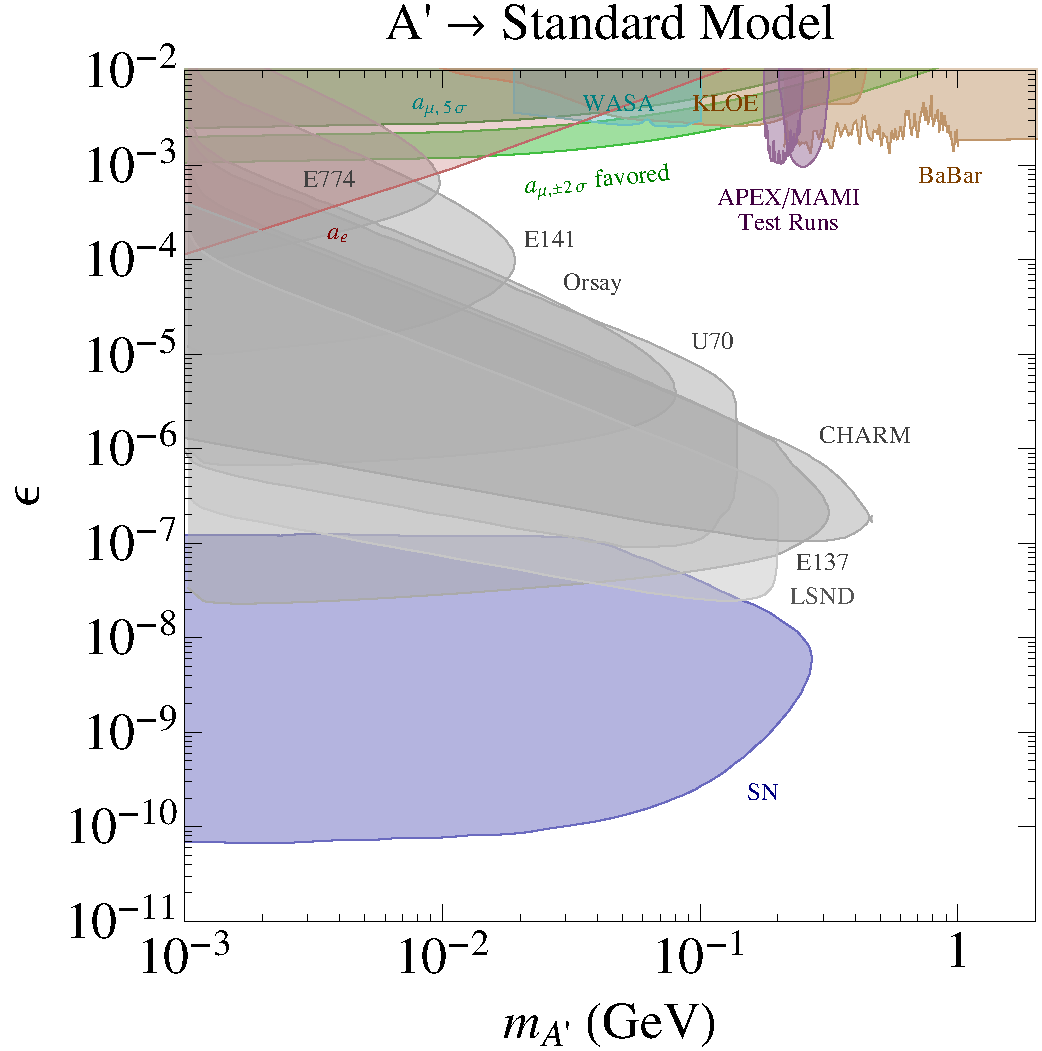
\includegraphics[width=0.48\textwidth,trim=0 0 0 1.8em,clip]{A-visible-large}
    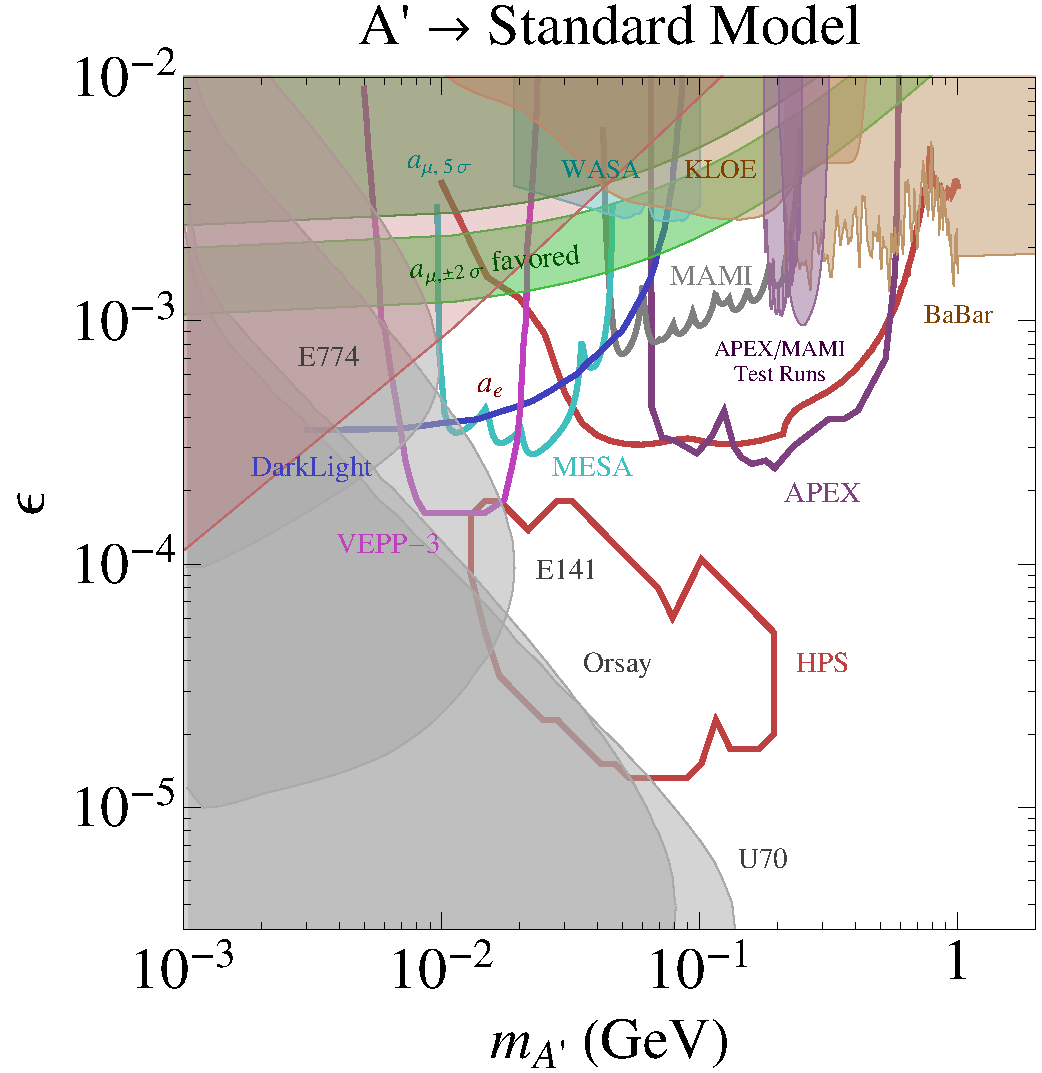
\includegraphics[width=0.48\textwidth,trim=0 0 0 1.8em,clip]{A-visible-zoom}
    \caption[Dark photon parameter space]
    {
      Parameter space for dark photons, $A^\prime$, with a mass above $1\mev$ showing the $90\pc$
      confidence level limits from numerous experiments.
      The right-hand panel is a zoom in of the left-hand panel, at low $\epsilon$; where
      the parameter $\epsilon$ characterizes the mixing between the \sm photon and the
      dark photon.
      These plots are taken from Ref.~\protect\cite{Essig:2013lka}.
    }
    \label{fig:db:darkphotonlimits}
  \end{center}
\end{figure}


In principal, the following analysis is sensitive to any dark sector particle.
However, in practice other experiments have searched directly for dark bosons with mass independent
couplings using much larger data samples.
For example, the NA48/2 collaboration has searched for a dark photon directly in the decay
\decay{\piz}{\gamma\darkgamma}~\cite{CERNNA48/2:2015lha}, and the \babar collaboration have
searched for evidence in the decay $\decay{\ee}{\gamma\darkgamma}$~\cite{Lees:2014xha}.
However, these decays involve the direct production of a dark photon at tree level.
Figure~\ref{fig:db:feynman} shows a Feynman diagram of how the decay \btokstrdb might proceed;
it shows an \fcnc where the \db results from a coupling to a \tquark quark.
Therefore, searching for evidence of a \btokstrdb where \dbtomumu is particularly sensitive to
portals which couple strongly to mass.

%High energy \lhc experiments at the \lhc have put stringent limits on new $U(1)$ states under the
%assumption that the coupling of \darkgamma to \sm states is large.
%However, if the coupling of these states is weak then \darkgamma could be light.

\begin{figure}
  \begin{center}
    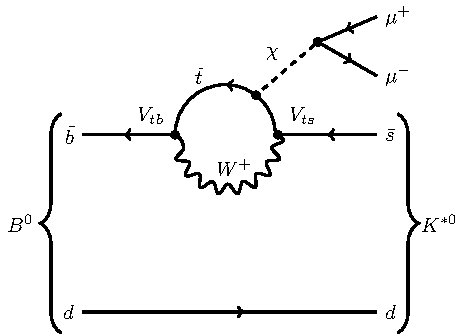
\includegraphics[scale=1]{feynman_inf}
    \caption[Feynman diagram for the decay \btokstrdb]
    {
      Feynman diagram showing the decay \btokstrdb, where the \db interacts by mixing with the
      Higgs or $Z$, which then decays into a dimuon pair.
    }
    \label{fig:db:feynman}
  \end{center}
\end{figure}


Na\"{i}vely, one might expect that because the \Bp is a pseudoscalar and the \Kstarz is a vector
the decay \btokstrdb would be rather more sensitive to a vector \d than one which is a scalar.
One might also conclude that to look for a vector \db, a better decay channel in which to search
would be \decay{\Bp}{\Kp\mumu}; despite its added experimental difficulties.
However, simply counting possible spin states that a two body decay can have, leads to the
conclusion that there should only a factor of about three between their branching fractions.
The angular momentum barrier only becomes significant when the phasespace for a decay begins
to be restricted.
Figure~\ref{fig:db:kx} shows the differences in branching fraction for \btokstrdb and
\decay{\Bp}{\Kp\db} where \db is a scalar and an pseudoscalar particle.
%; the decay rate predictions
%are taken from an axion portal model in Ref~\cite{Batell:2009jf}.
Decay rate predictions for a \db operating through the axion portal for decays of the type
\decay{B}{K\db} to be~\cite{Batell:2009jf}:
\begin{align}
  \Gamma\big(\decay{B}{K\db}\big) &= \Gamma_0
  \frac{\lambda_{K}\big(m_{B}^2-m_{K}^2\big)^2}{m_{B}^6}
  \left[f_0\!\left(m_\db^2\right)\right]
  \\
  \Gamma\big(\decay{B}{\Kstar\db}\big) &= \Gamma_0
  \frac{\lambda_{\Kstar}^3}{m_{B}^6}
  \left[A_0\!\left(m_\db^2\right)\right]
  \\
  \intertext{where the phasespace factor is}
  \lambda_\kappa &= \left[
    \left( m_B^2 - m_\db^2 - m_\kappa^2 \right)^2
    -4m_\db^2m_\kappa^2
    \right]^\frac12,
    \label{eq:db:bx}
\end{align}
form factors are denoted as $f_0$ $A_0$, and $\Gamma_0$  is a constant.
Figure~\ref{fig:db:kx} shows that the phasespace factor is the dominant factor in the shape for all
the decays, and that searching for a particle, \db, in the decays \decay{\Bd}{\Kstarz\db} and
\decay{\Bp}{\Kp\db} is similarly sensitive for $m_\db\lesssim2000\mev$.

\begin{figure}
  \begin{center}
    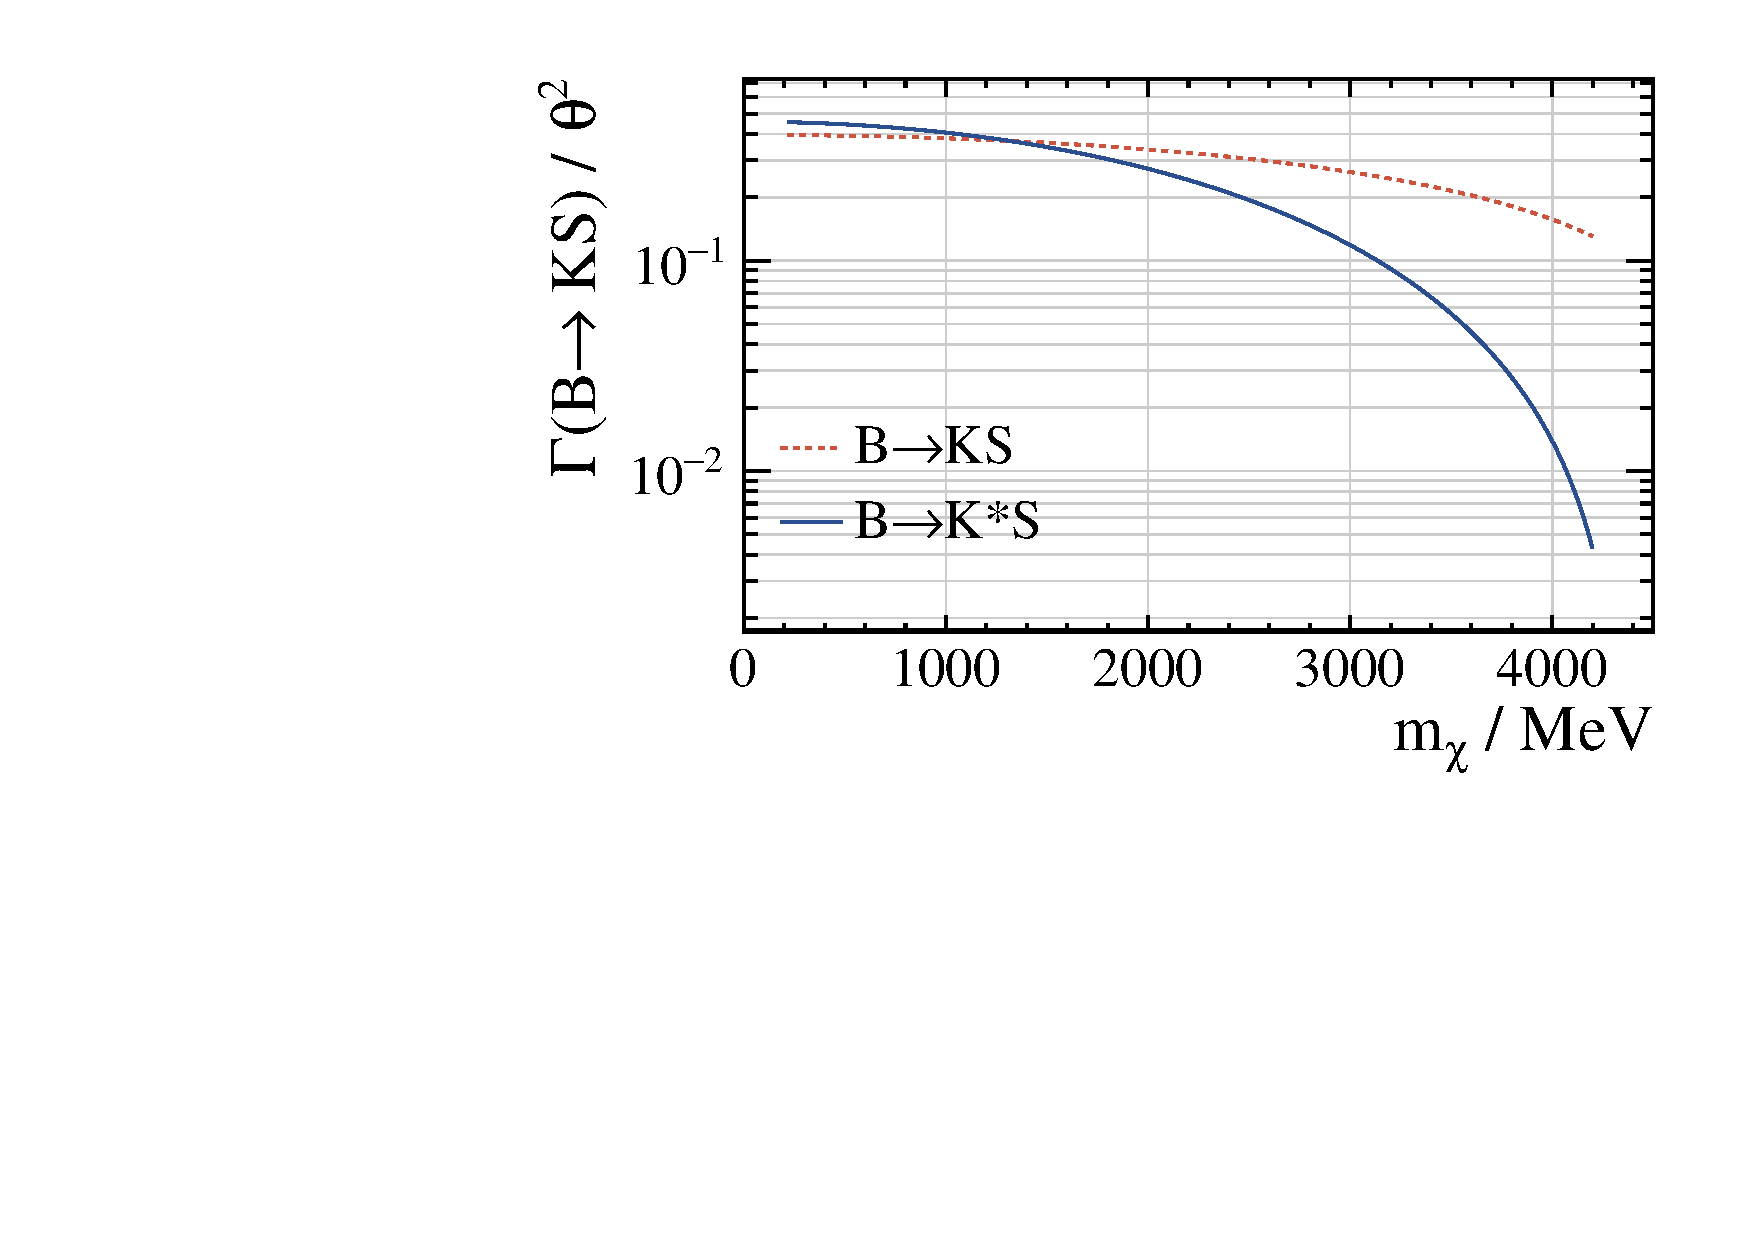
\includegraphics[width=0.48\textwidth]{bf_b2ks_root}
    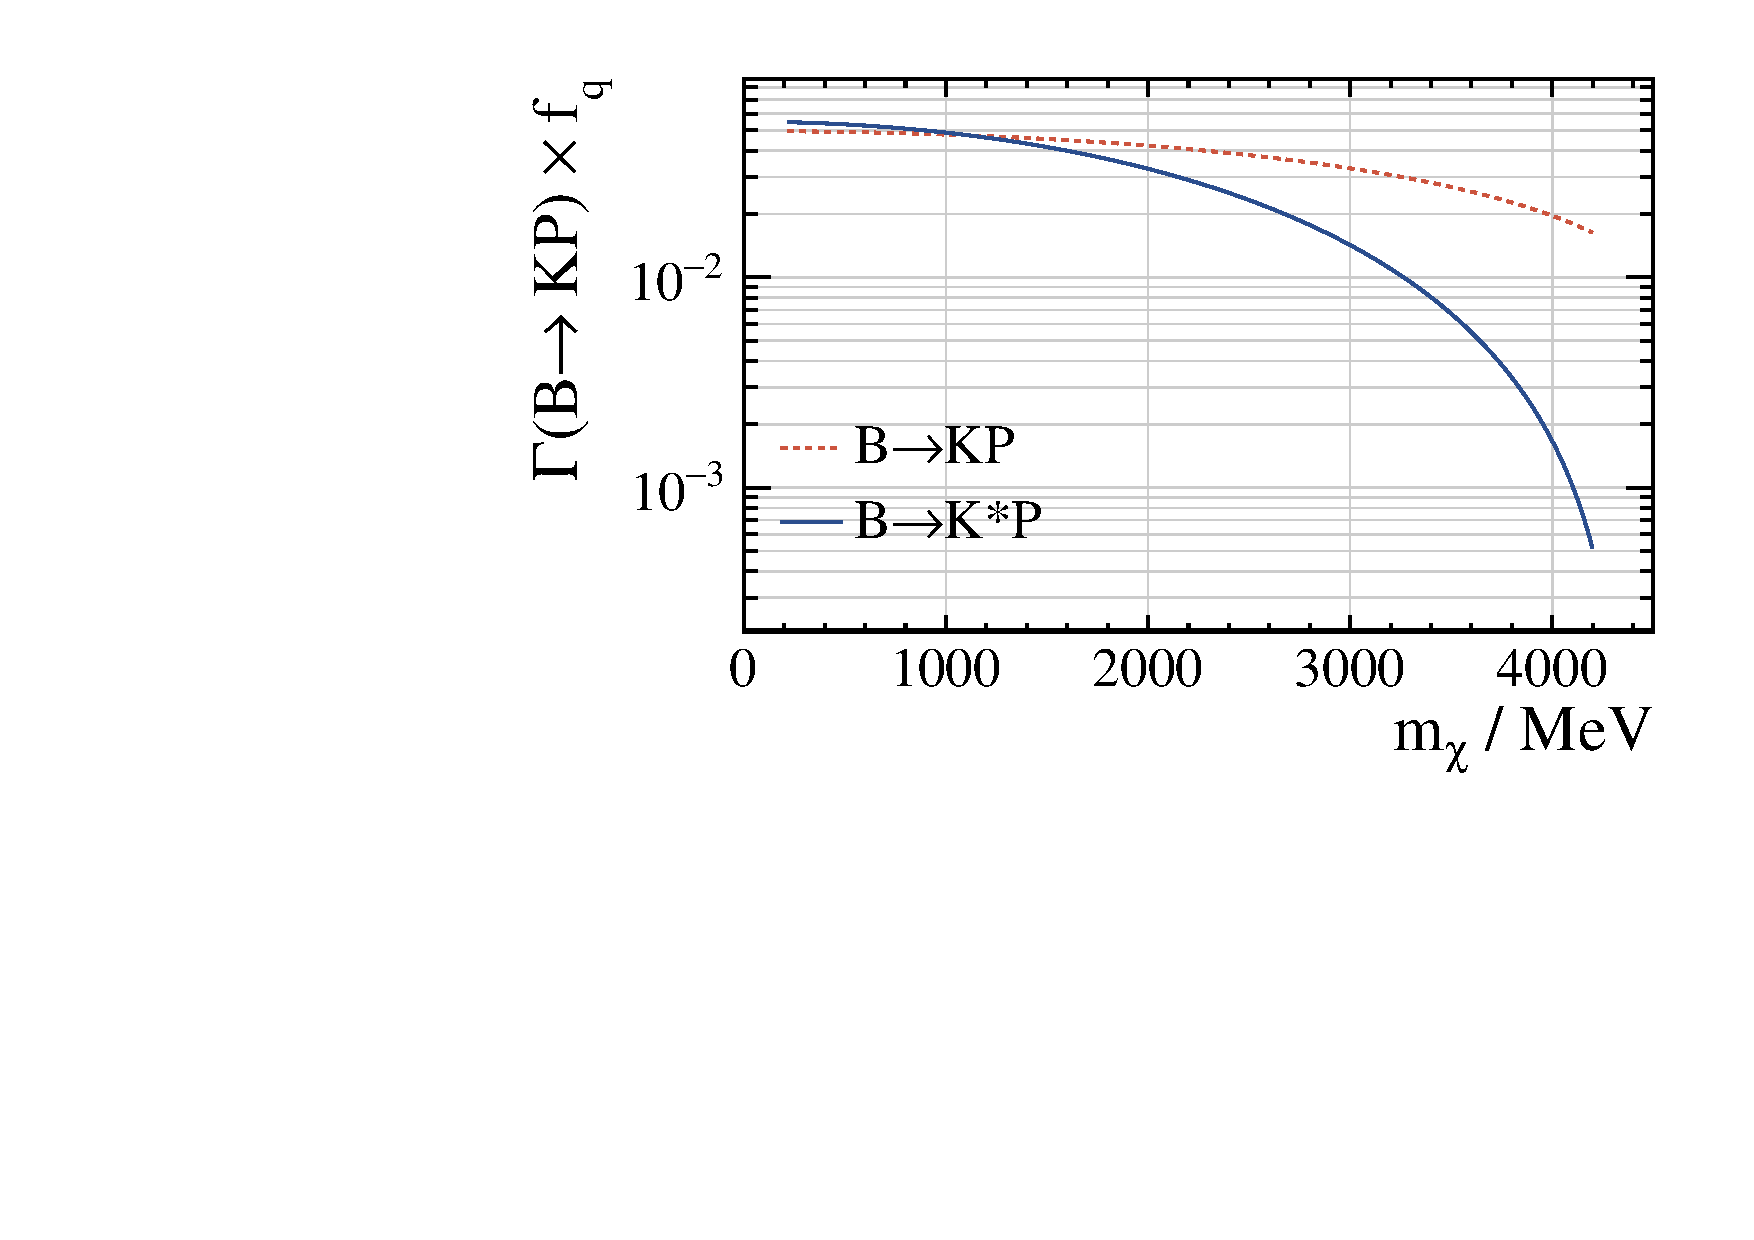
\includegraphics[width=0.48\textwidth]{bf_b2kv_root}
    \caption[Decay rates for decays of the form \decay{B}{K\db}]
    {
      Decay rate predictions, from Eq.~\protect\ref{eq:db:bx},
      for decays of the form $\decay{B}{KX}$, where $X$ is either
      (left) a scalar (S) or
      (right) an axial-vector (A).
      The parameters $\theta$ and $f_q$ are parameters of the model in
      Ref~\cite{Batell:2009jf}.
      The shapes of the curves are dominated by the available phasespace, and sensitivity is
      comparable for $m_\db\lesssim2000\mev$.
    }
    \label{fig:db:kx}
  \end{center}
\end{figure}


The following chapter introduces an analysis strategy, an overview of the selection, and how the
discrete samples of \btokstrdb are used to parameterize all masses.



%Many extensions of the SM predict the existence of a new light boson.
%As all interactions in the SM are gauged, it is reasonable to assume that the same can be said of
%interactions in the dark sector.
%If so, then they would contain new vector bosons such as so-called dark photons (referred to as
%$A^{\prime}$), dark $Z$ bosons (referred to as $Z_d$).
%%A particular model that would anticipate the observation of a light vector boson would one which
%%includes a dark $Z$ (or photon).
%%Such models are motivated by the existence of dark matter and also the $3.6\,\sigma$ deviation
%%exhibited between the theoretical and experimental measurements of the anomalous magnetic moment of
%%the muon, $a_\mu=\tfrac12(g_\mu-2)$~\cite{PDG2012}.
%A $Z_d$ that weakly couples to the visible sector with low mass
%($10\lesssim m_{Z_d}\lesssim500\mev$) would add corrections to the theoretical value of $a_\mu$
%bringing it in line with what is seen experimentally.
%Such models are outlined in Refs.~\cite{Davoudiasl:2012qa,Davoudiasl:2012ag,Lee:2014lga}.
%%Other models might include such particles as Inflatons~\cite{Bezrukov:2009yw} and
%%Axions~\cite{Peccei:2006as}.
%Other models include the Pecci-Quinn axion~\cite{PhysRevLett.38.1440}, as described in \Sec{ch:th},
%which solves the strong \CP problem by the addition of a pseudoscalar axion particle.



%In general, extensions to the SM include bosons that couple to fermions proportionally to
%their masses.
%This occurs either due to mixing with the SM Higgs boson or due to the fact that the
%new bosons arise via a symmetry breaking process similar to the Higgs mechanism.
%Therefore, processes that are mediated via loops that contain top quarks are excellent places to
%search for such particles.



%The spin of the particle is not assumed either.
%A similar analysis might search for a \db in \decay{\Bp}{\Kp\mumu}, where one might expect
%additional sensitivity to scalar particles.
%However, this is not the case.
%Reference~\cite{Batell:2009jf} gives decay rates for decays of the type \decay{B}{K\db} to be:
%\begin{align}
  %\Gamma\big(\decay{B}{K\db}\big) &= \Gamma_0
  %\frac{\lambda_{K}\big(m_{B}^2-m_{K}^2\big)^2}{m_{B}^6}
  %\left[f_0\!\left(m_\db^2\right)\right]
  %\\
  %\Gamma\big(\decay{B}{\Kstar\db}\big) &= \Gamma_0
  %\frac{\lambda_{\Kstar}^3}{m_{B}^6}
  %\left[A_0\!\left(m_\db^2\right)\right]
  %\\
  %\intertext{where the phasespace factor is}
  %\lambda_\kappa &= \left[
    %\left( m_B^2 - m_\db^2 - m_\kappa^2 \right)^2
    %-4m_\db^2m_\kappa^2
    %\right]^\frac12,
    %\label{eq:db:bx}
%\end{align}
%form factors are denoted as $f_0$ $A_0$, and $\Gamma_0$  is a constant.
%Figure~\ref{fig:db:kx} shows that the phasespace factor is the dominant factor in the shape for all
%the decays, and that searching for a particle, \db, in the decays \decay{\Bd}{\Kstarz\db} and
%\decay{\Bp}{\Kp\db} is equally sensitive for $m_\db\lesssim2000\mev$.
%%For example, Fig.~\ref{fig:th:kx} shows how the branching fraction of \decay{\Bd}{\Kstar\db} is
%%expected to vary with the mass of the \db, in comparison to \decay{\Bd}{K\db}.

%\begin{figure}
  %\begin{center}
    %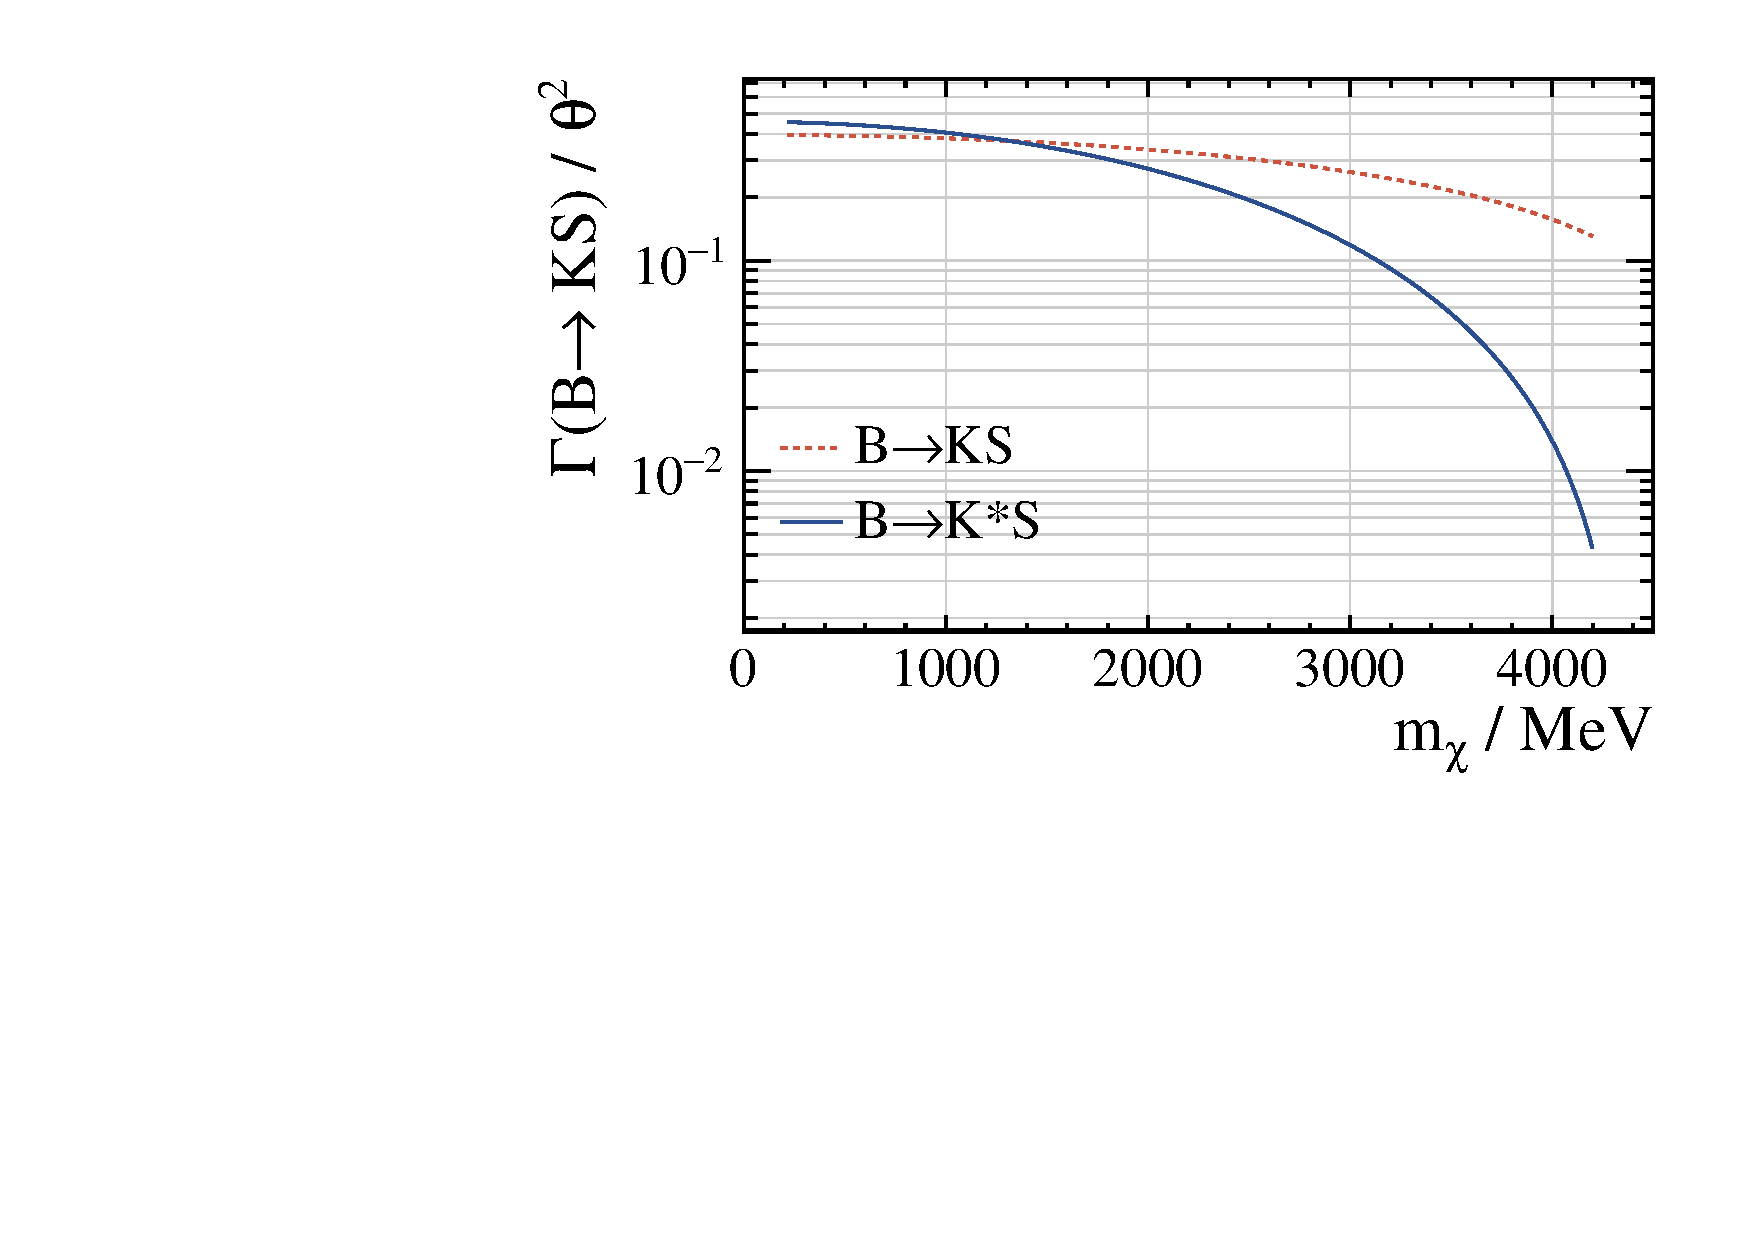
\includegraphics[width=0.48\textwidth]{bf_b2ks_root}
    %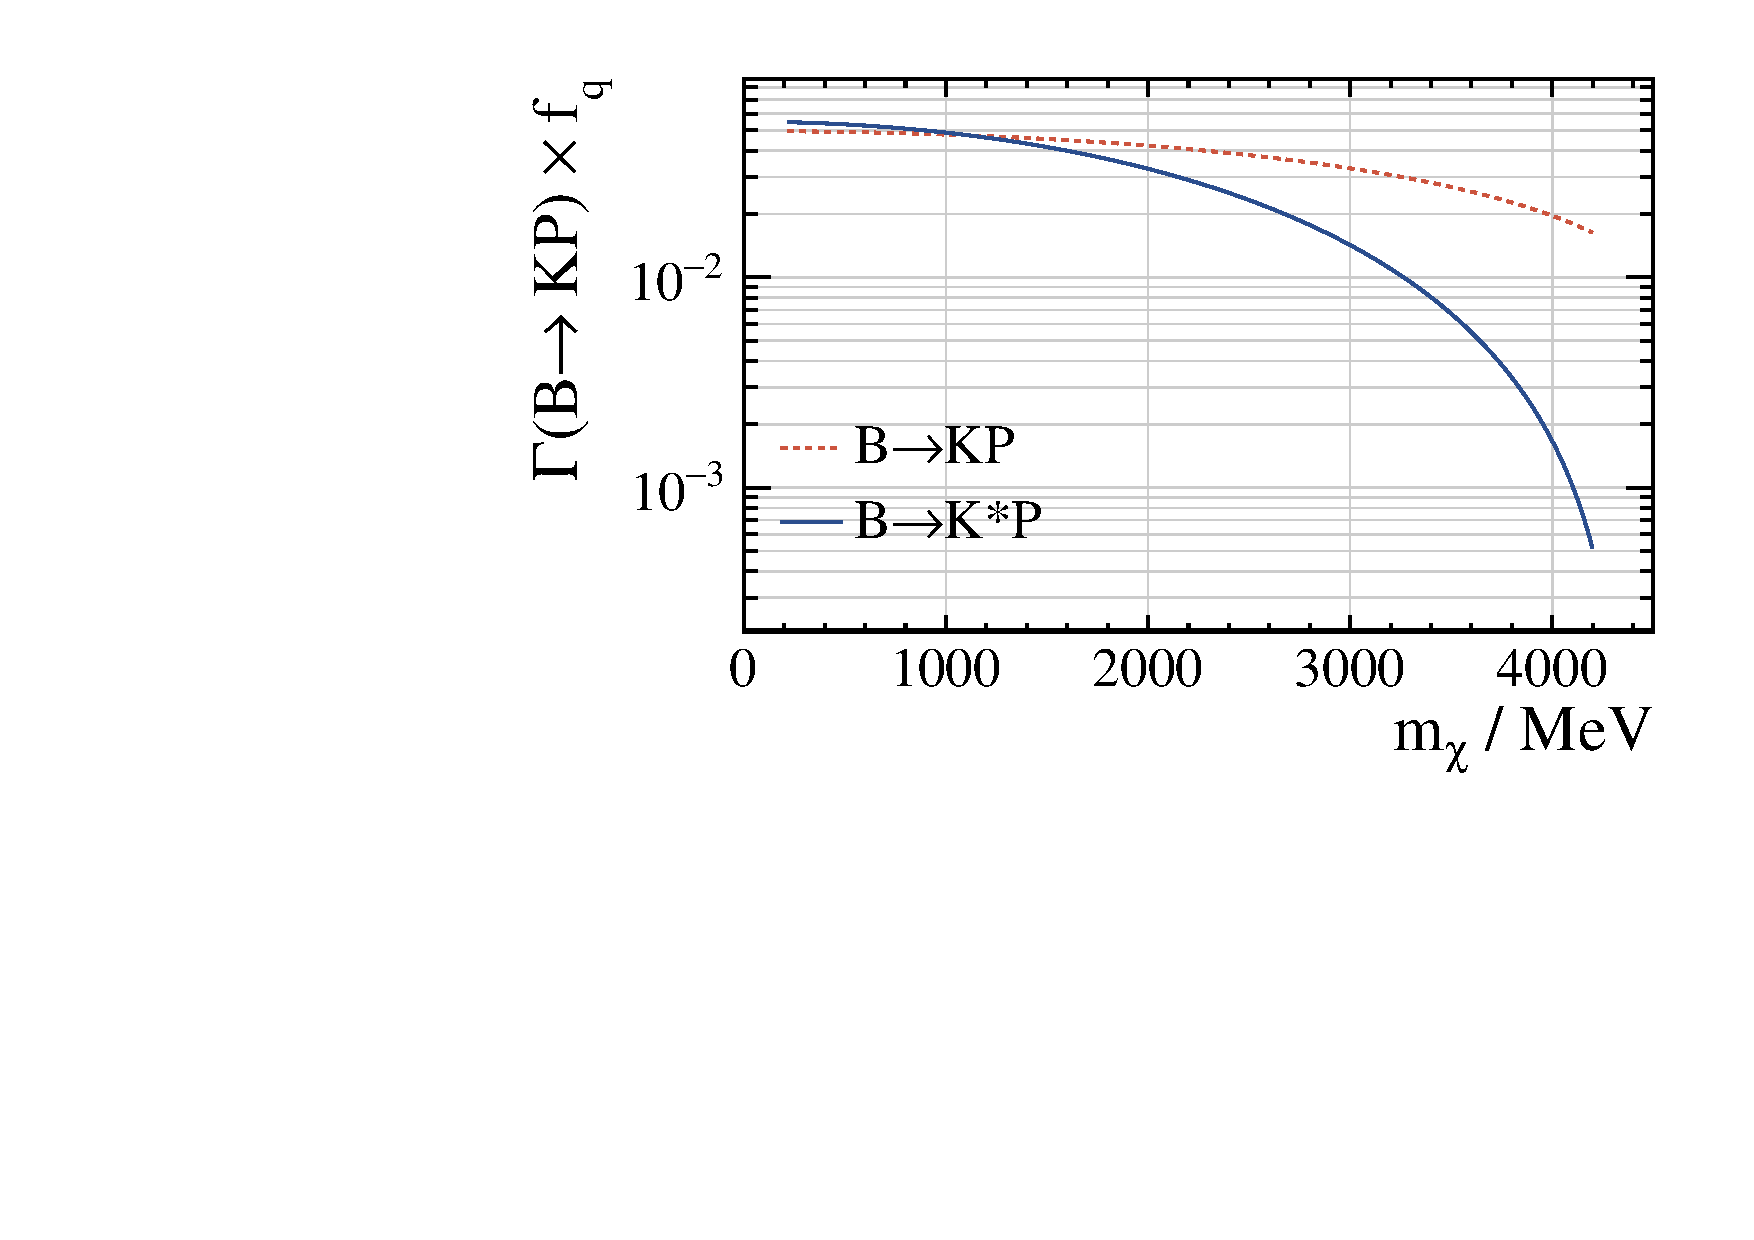
\includegraphics[width=0.48\textwidth]{bf_b2kv_root}
    %\caption{
      %Branching fraction predictions, from Eq.~\protect\ref{eq:db:bx},
      %for decays of the form $\decay{B}{KX}$, where $X$ is either
      %(left) a scalar (S) or
      %(right) a vector (V).
      %The parameters $\theta$ and $f_q$ are parameters of the model.
      %%Note that for these plots $\mathrm{ln}\left(\Lambda_\mathrm{UV}/m_t\right)$ is set to one.
      %The shapes of the curves are dominated by the available phasespace, and sensitivity is
      %comparable for $m_\db\lesssim2000\mev$.
      %%this is taken from Ref~\cite{Batell:2009jf}.
    %}
    %\label{fig:db:kx}
  %\end{center}
%\end{figure}


%The following analysis is a fully frequentist search for a new particle \db, with an unknown mass
%ans lifetime.
%This is done in the two dimensions of mass and lifetime using the method described in
%\Sec{sec:db:strategy}.



%%%%%%%%%%%%%%%%%%%%%%%%%%%%%%%%%%%%%%%%%%%%%%%%%%%%%%%%%%%%%%%%%%%%%%
% NOTHING BEYOND HERE
%%%%%%%%%%%%%%%%%%%%%%%%%%%%%%%%%%%%%%%%%%%%%%%%%%%%%%%%%%%%%%%%%%%%%%


%The existence of dark matter in the universe is overwhelmingly supported by experimental evidence from galactic rotation curves, gravitational lensing, and acoustic modes in the CMB.
%As there are no viable dark matter candidate particles in the Standard Model (SM), new {\em dark} particles must exist.
%Dark matter provides strong evidence for a \emph{dark sector}, containing particles which only
%interact weakly with the spectrum of SM particles via mediating messenger particles, or
%\emph{Dark Bosons}.
%%Despite the countless successes of the Standard Model (SM), it is well known that it is an
%%incomplete picture of particle physics, failing, as it does, to explain a number of important
%%phenomena.
%%These range from theoretical problems of naturalness to experimental indications of Dark matter.
%%All of these point towards the existence of beyond SM physics, and the existence of an, as yet,
%%undiscovered particle.
%The following analysis note details the search for a hypothetical Dark Boson, \db, of
%unknown mass and lifetime.

%Many extensions of the SM predict the existence of a new light boson.
%As all interactions in the SM are gauged, it is reasonable to assume that the same can be said of
%interactions in the dark sector.
%If so, then they would contain new vector bosons such as so-called dark photons (referred to as
%$A^{\prime}$), dark $Z$ bosons (referred to as $Z_d$).
%%A particular model that would anticipate the observation of a light vector boson would one which
%%includes a dark $Z$ (or photon).
%%Such models are motivated by the existence of dark matter and also the $3.6\,\sigma$ deviation
%%exhibited between the theoretical and experimental measurements of the anomalous magnetic moment of
%%the muon, $a_\mu=\tfrac12(g_\mu-2)$~\cite{PDG2012}.
%A $Z_d$ that weakly couples to the visible sector with low mass
%($10\lesssim m_{Z_d}\lesssim500\mev$) would add corrections to the theoretical value of $a_\mu$
%bringing it in line with what is seen experimentally.
%Such models are outlined in Refs.~\cite{Davoudiasl:2012qa,Davoudiasl:2012ag,Lee:2014lga}.
%Other models might include such particles as Inflatons~\cite{Bezrukov:2009yw} and
%Axions~\cite{Peccei:2006as}.

%Many beyond SM regimes include a new boson which, as a result of electroweak symmetry breaking or a
%similar mechanism, couple to fermions proportionally to their mass.
%%In general, extensions to the SM often include bosons that couple to fermions proportionally to
%%their masses.
%%This occurs either due to mixing with the SM Higgs boson or due to the fact that the
%%new bosons arise via a symmetry breaking process similar to the Higgs mechanism.
%Therefore, processes that are mediated via loops that contain top quarks are excellent places to search for such particles.
%Figure~\ref{fig:feynman} shows a Feynman diagram of a potential process.
%
%\begin{figure}
  %\begin{center}
    %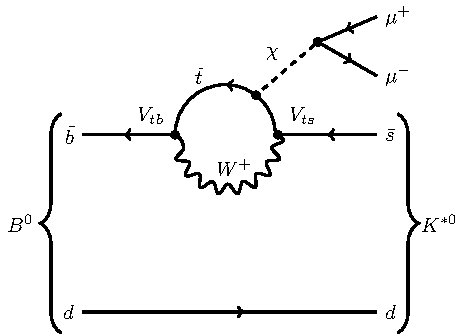
\includegraphics[scale=1]{feynman_inf}
  %\caption{
    %Feynman diagram showing the decay \btokstrdb, where the \db interacts by mixing with the
    %Higgs or $Z$, which then decays into a dimuon pair.
  %}
  %\label{fig:feynman}
%\end{center}
%\end{figure}

%%Many models which propose such a particle, but generally (for $m<m(B)$) they are dark
%%sector particles and only interact with the visible sector by mixing with the Higgs or $Z$ boson.
%%Some general theories predict particles known as:
%%\begin{itemize}
  %%\item Axions
  %%\item Any other generic beyond SM particle.
%%\end{itemize}
%
%In this analysis, a \db is searched for in the decay
%$\Bd\!\to K^*(892)^0\infl$, where $\Kstarz\!\to\Kp\pim$ and $\infl\!\to\mumu$
%(charge conjugation is assumed throughout this document, and unless explicitly
  %stated otherwise, $K^{*0}$ refers to the $K^*(892)^0$).
%The analysis is general in that no mass, lifetime or spin is assumed for \db.
%%This search is sensitive to both vector and scalar particles.
%For example, Fig.~\ref{fig:th:kx} shows how the branching fraction of \decay{\Bd}{\Kstar\db} is
%expected to vary with the
%mass of the \db, in comparison to \decay{\Bd}{K\db}.
%This is the case for a scalar or vector \db.
%
%In the dimuon mass region below the $J/\psi$ mass, both the $K$ and \Kstar decay modes are roughly
%equally sensitive to vector and scalar particles.
%%Appendix~\ref{app:np} provides more details on beyond the SM theories which include a particle
%%that this search could be sensitive to.
%
%\begin{figure}
  %\begin{center}
    %\subfloat[\label{fig:th:ks}]{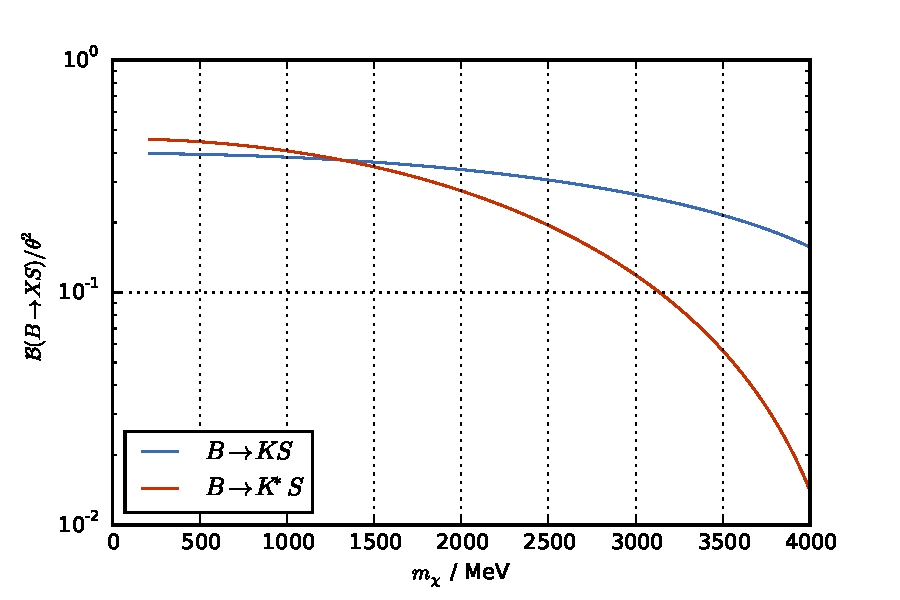
\includegraphics[width=0.48\textwidth]{bf_b2ks}}
    %\subfloat[\label{fig:th:kv}]{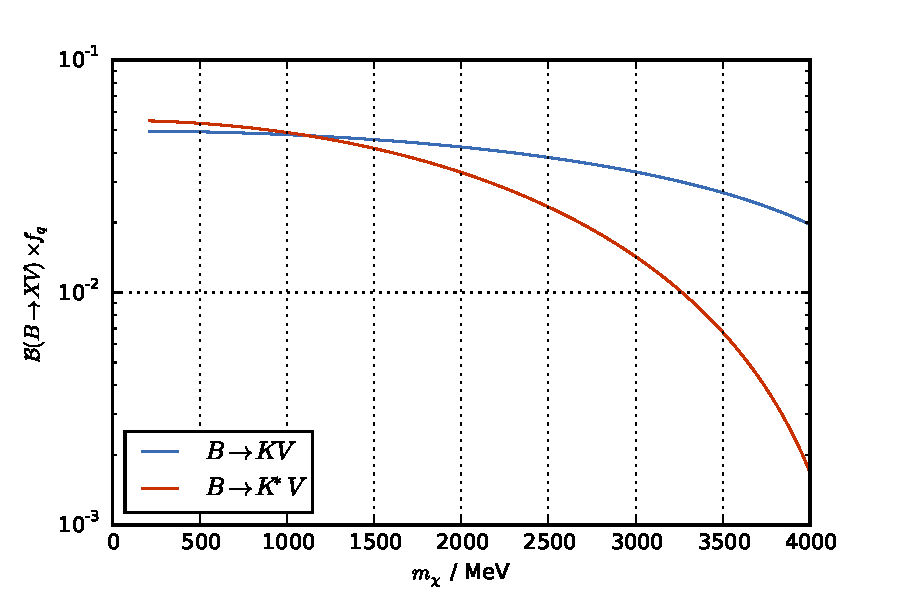
\includegraphics[width=0.48\textwidth]{bf_b2kv}}
    %\caption{
      %Branching fraction distributions %from Eq.~\protect\ref{eq:th:bx}
      %for $\decay{B}{KX}$ where $X$ is either
      %\protect\subref{fig:th:ks} a scalar (S) or
      %\protect\subref{fig:th:kv} a vector (V).  Note that for these plots
      %$\mathrm{ln}\left(\Lambda_\mathrm{UV}/m_t\right)$ is set to one.
      %The shapes of the curves are dominated by the available phasespace, this is taken
      %from Ref~\cite{Batell:2009jf}.
    %}
    %\label{fig:th:kx}
  %\end{center}
%\end{figure}
%
%
%
%
%\section{New physics scenarios}
%\label{app:np}
%
%\subsection{New scalar particles}
%In this search we are looking for $\decay{\Bd}{K^*(892)^0\db}$, and since the \Bd is a
%psuedoscalar, and
%the $K^*(892)^0$ is a vector; nai\"{i}vely one might expect that the \db must also be a vector.
%However, this is not the case.
%The equations given in Ref.~\cite{Batell:2009jf}:
%\begin{align}
  %\BF(\decay{B}{KS})
  %&=4\e{-7}\times\left(\frac{\theta}{10^{-3}}\right)^2
  %\mathcal{F}_K^2(m_S)\lambda^\frac12_{KS} \nonumber\\
  %\BF(\decay{B}{K^*S})
  %&=5\e{-7}\times\left(\frac{\theta}{10^{-3}}\right)^2
  %\mathcal{F}_K^{*2}(m_S)\lambda^\frac32_{K^*S} \nonumber\\
  %\BF(\decay{B}{KV})
  %&=5\e{-6}\times
  %\left[ \frac{100\tev}{f_q}\mathrm{ln}\left(\frac{\Lambda_\mathrm{UV}}{m_t}\right) \right]^2
  %\mathcal{F}_K^2(m_V)\lambda^\frac12_{KV} \nonumber\\
  %\BF(\decay{B}{K^*V})
  %&=6\e{-6}\times
  %\left[ \frac{100\tev}{f_q}\mathrm{ln}\left(\frac{\Lambda_\mathrm{UV}}{m_t}\right) \right]^2
  %\mathcal{F}_K^2(m_V)\lambda^\frac32_{K^*V} \nonumber
  %\label{eq:th:bx}
%\end{align}
%where
%\begin{equation}
  %\lambda_{ij} = \frac{1}{m_B^4}
  %\left(m_b^2 - \left(m_i+m_j\right)^2\right)
  %\left(m_b^2 - \left(m_i-m_j\right)^2\right)
%\end{equation}
%is the phasespace term and $\mathcal{F}$ are form factors.
%Branching fraction distributions for the scalar and vector dark bosons are shown in
%\Fig{fig:th:kx}, these show that the branching fraction for the $K^*$ mode is greater for
%$m_\db\lesssim1250\mev$ compared to the $K$ mode.
%
%
%\subsection{Axions}
%A gauge invariant term that can be added to $\Lag{QCD}$ is
%\begin{equation}
  %\Lag{QCD}^\theta = \theta\frac{g^2}{32\pi^2}
  %F_{\mu\nu}^\alpha\widetilde F^{\mu\nu}_\alpha,
%\end{equation}
%where $\theta$ and $g$ are constants, and $\alpha$ indicates a sum over colours.
%The operator $F_{\mu\nu}$ is the gluon field strength tensor, and
%\begin{equation}
  %\widetilde F^{\mu\nu}_\alpha = \frac12\varepsilon_{\mu\nu\rho\sigma}F^{\rho\sigma}_\alpha.
%\end{equation}
%An interaction such $\Lag{QCD}^\theta$ would conserve charge symmetry, but violate parity and time
%conjugation~\cite{Peccei:2006as}.
%Such symmetry violations are in contradiction with the observed properties of the strong
%force.
%Bounds placed on the value of the neutron dipole moment, $|d_n| <2.9\e{-26}\,\mathrm{ecm}$
%(at 90\% CL)~\cite{Baker:2006ts} requires $\theta$ to be very small,
%$\theta<10^{-19}$~\cite{Crewther:PQref9}, when \emph{a priori} it could be in the range
%$0<\theta<2\pi$.
%This occurrence of fine tuning is referred to as the \emph{strong CP problem}.
%A solution to this problem is to introduce an additional chiral symmetry, such that $\theta$
%becomes a field, the quanta of which are called axions.
%%A solution of the strong CP problem is to introduce a chiral $U(1)$ symmetry which is spontaneously
%%broken and effectively replaces the CP violating angle $\theta$ with a CP conserving field.



%\subsection{Inflatons}
%Cosmological inflation in the early universe (very early, $t=10^{-35}$ to $10^{-34}$\,s can be put
%down to the existence of a scalar field that weakly couples to SM particles via some mixing with the
%Higgs sector.
%Before expansion, the inflation field was at a higher energy state.
%Quantum fluctuations caused a phase transition where the inflaton field released its potential
%energy as matter radiation as it settled to its lowest energy state,
%This action generated a repulsive force that drove the portion of the universe that is observable
%today to accelerate in expansion.
%Many of such theories predict the mass of the scalar to be massive, potentially beyond the reach of
%the \lhc.
%However, there is hope, Ref.~\cite{Bezrukov:2009yw} outlines possibilities for the inflaton to be in
%the range $270 < m(\infl) < 10000$\mev.
%
%This model has a Lagrangian which looks like:
%\begin{align}
  %\Lag{tot} &= \Lag{SM} + \Lag{\db} \\
  %\Lag{\db} &= \frac12\partial_\mu\infl\partial^\mu\infl
  %+\frac12m(\infl)^2\infl^2
  %-\frac\beta4\infl^4
  %-\lambda\left(H^\dagger H-\frac\alpha\lambda\infl^2\right)^2.
  %\label{eq:laginf}
%\end{align}
%Where the term $\Lag{SM}$ is the SM Lagrangian without the Higgs potential, which gets
%modified to that shown in Eq.~\ref{eq:laginf}



